\documentclass[12pt,letterpaper]{article}
\usepackage{color,amsmath,amsthm,amsfonts,graphicx,float,units,subfig,subfloat,anysize}
\marginsize{2cm}{2cm}{2cm}{2cm}
\DeclareGraphicsExtensions{.pdf,.png,.jpg}
\graphicspath{{./images/}}
\begin{document}

\title{HCIPlayer: User Manual}
\author{ECSE424 Winter 2010, McGill University}
\renewcommand{\today}{Updated: Wednesday, March 24th, 2010}
\maketitle

\begin{center}
{\color{green} Green} sections indicate improvement suggested by the TA \\
{\color{magenta} Magenta} sections indicate improvement suggested by the team E-Mall \\
{\color{blue} Blue} sections indicate new features
\end{center}

\section{Introduction}

HCIPlayer is a portable music player which can be controlled either by using gestures or by speaking commands. It is implemented as an iPhone application using the user's own music library through the builtin iPod music player.

This user manual provides a detailed description of the available system functions, and will be updated as more features are implemented.

\section{Starting The Application}
First, if a high-speed WIFI network is available, connecting to it will provide a substantial performance boost. To start the application, select the \emph{HCI Music Player} icon on the iPhone main menu. The necessity of a visual icon is a byproduct of the chosen prototype environment and is intended for use by the evaluators only. The system will load to normal startup after the \emph{HCI Music Player} icon has been pressed.
\begin{itemize}
\item If this is the first time a user is starting the software, then an introductory tutorial on how to use the Player will begin as soon as the application has finished loading properly. This tutorial starts by explaining that if the user wishes to skip the tutorial he/she should double-tap the screen as instructed, then it explains the core functionality of the Player. {\color{blue} The tutorial can be listened to again at any later time by saying ``Tutorial'' as a voice command.}
\end{itemize}

\section{Player Operation}
	
HCIPlayer implements a simple and relatively common playlist-based music player. This is centered around the concept of a \emph{playlist}, which is an ordered list of \emph{tracks} from the \emph{music library} (which is itself a playlist). At any given time, there is an \emph{active playlist}, from which tracks are played in sequence. When HCIPlayer starts, the user's last-active playlist is set as the active playlist. The player also supports \emph{playback shuffle} (which plays the tracks in a random order) and \emph{playback repeat} (which repeatedly plays the current track or playlist).

When the player starts up and has loaded successfully, it will vibrate 4 times, {\color{magenta} say ``hello''}, and display a ``play'' icon.


\subsubsection*{Gestures}
HCIPlayer supports several gestures which can control music playback. These gestures are performed by tapping or sliding fingers on the touch surface. A \emph{tap-and-swipe} gesture refers to a quick tap followed by a longer swipe or drag starting from the same location.
\subsubsection*{Voice Commands}
To issue a voice command, place a finger on the touch surface until the full command has been spoken. A vibration will indicate that the HCIPlayer is ready to accept a voice command. If, for some reason or another, the voice command is taking a particularly long time to process, {\color{magenta}this will be indicated by a circle moving around the center of the screen}, as well as periodic vibration.

\begin{figure}[H]
	\centering
	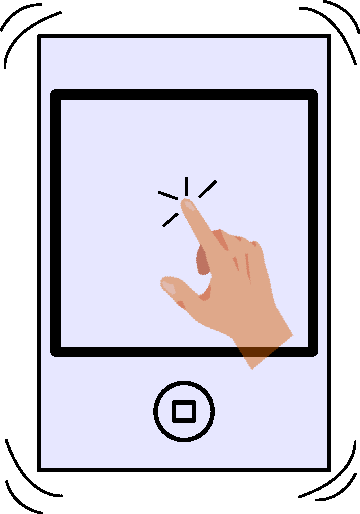
\includegraphics[scale=0.6]{touch}
	\caption{Touch \& hold until vibration \\ Enable speech recognition to issue a voice command}
\end{figure}
\subsection*{Playback}
The \textbf{play} or \textbf{pause} actions can be signalled in a number of ways:
\begin{itemize}
\item A single short tap causes the current track to start playing, or if it is already playing, causes the playback to pause.
\item Issuing the voice command `play' or `pause' will perform the desired operation.
\item The play command allows for a specific artist, album, or song to be selected for immediate playback. \\ The following may also be used in any combination to play a specific item or set of items in the music collection:
	\begin{itemize}
	\item Play artist \textit{ARTIST}
	\item Play album \textit{ALBUM}
	\item Play track or song \textit{TRACK}
	\end{itemize}
\end{itemize}
\textbf{Stop} may be signalled by issuing the `stop' voice command.
\subsubsection*{Queueing}
Similar to how songs are selected for immediate playback, they can also be appended to the current playlist using the \textbf{queue} command. To \textbf{queue} an artist, album, or song, issue the any combination of the following commands:
	\begin{itemize}
	\item Queue artist \textit{ARTIST}
	\item Queue album \textit{ALBUM}
	\item Queue track or song \textit{TRACK}
	\end{itemize}
\subsubsection*{Volume}
Volume is adjusted by swiping up and down accordingly on the screen. \\
{\color{green} There also used to be a \textbf{mute} function, but this has been obsoleted by the \textbf{pause} function.}
\subsubsection*{Seeking}
To navigate through the current track, tap the screen and then drag right or left to \textbf{fast-forward} or \textbf{rewind} respectively.
\subsubsection*{Replay}
To restart playback of the current song (\textbf{replay}), issue the voice command `replay'.


\subsection*{Playlist Navigation}
Navigation to the \textbf{previous} or \textbf{next} track is performed by a swiping gesture accross the surface of the player.
	\begin{figure}[H]
		\centering
		\subfloat[][Swipe left -- \textbf{Previous} track]{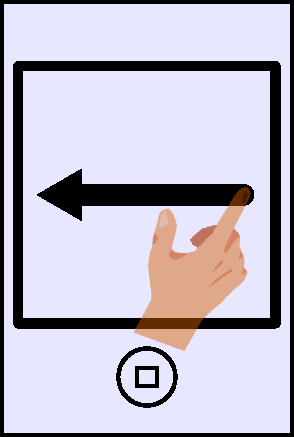
\includegraphics[scale=0.6]{left20}}
		\hspace{1in}
		\subfloat[][Swipe right -- \textbf{Next} track]{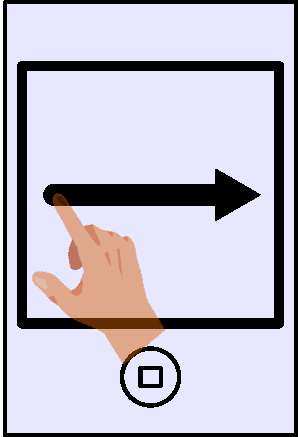
\includegraphics[scale=0.6]{right20}}
		\caption{Navigation gestures}
	\end{figure}
{\color{green}NOTE: The gestures used to be reversed} \\
Alternately, the same effect will be achieved by issuing the voice commands, `previous' or `next'. \\
\subsubsection*{Shuffle}
The \textbf{shuffle} mode allows for the playlist to, rather than following the prescribed ordering, randomly select each next song. This mode can be toggled by the voice commands `shuffle' or `toggle shuffle'. Alternately it may be set by the commands, `shuffle on/off' or `turn shuffle on/off'. The \emph{alpha} ($\alpha$) gesture also toggles the \textbf{shuffle} mode:
\begin{figure}[H]
	\centering
	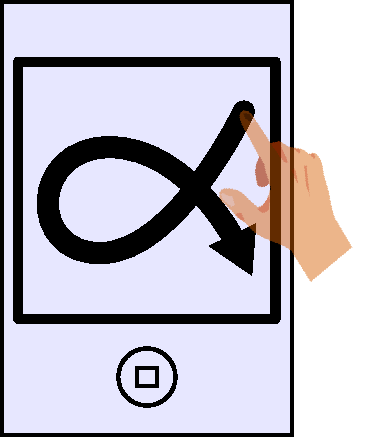
\includegraphics[scale=0.6]{alpha}
	\caption{\emph{Alpha} gesture -- Toggle \textbf{shuffle} mode}
\end{figure}
\subsubsection*{Repeat}
The \textbf{repeat} mode allows for a playlist to repeat itself upon completion. Similar to the \textbf{shuffle} command, \textbf{repeat} can be toggled by the voice commands `repeat' or `toggle repeat'. It may also be set by the commands `repeat on/off' or `turn repeat on/off'. The corresponding \emph{circle} gesture also toggles the \textbf{repeat} mode:
\begin{figure}[H]
	\centering
	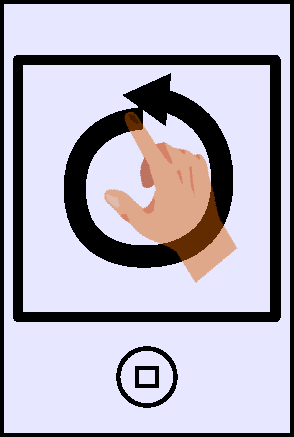
\includegraphics[scale=0.6]{circle}
	\caption{\emph{Circle} gesture -- Toggle \textbf{repeat} mode}
\end{figure}

\subsection*{Feedback}
A number of commands exist to help the user figure out the system.
\subsubsection*{What's Playing?}
To find out what track is currently playing, give any of the voice commands `what's playing?', `info', `now playing',  or draw a \emph{question mark} on the screen:
\begin{figure}[H]
	\centering
	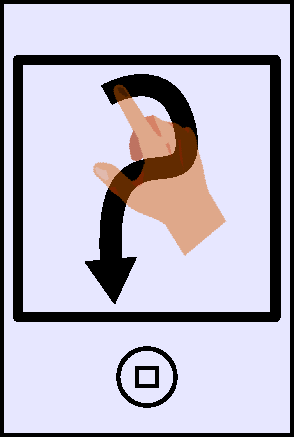
\includegraphics[scale=0.6]{question}
	\caption{\emph{Question mark} gesture -- What's playing?}
\end{figure}
\subsubsection*{Help!}
To get a list of available commands, say `help', `what can I say?', `list commands', or `help me'. \\
{\color{magenta}The voice command `tutorial' will start the new user tutorial.}

\end{document}
